\section{Microarchitecture overview}

The core is a five-stage RV32I pipeline (F/D/E/M/W). Instructions overlap in
flight; stage boundaries are defined by pipeline registers, and a dedicated
hazard unit generates forwarding, stall, and flush control.
The block schematics in this section (Figures~\ref{fig:uarch-system}--\ref{fig:uarch-execute})
are generated directly from the RTL with Yosys and \texttt{netlistsvg} (via
\texttt{scripts/gen\_schematic.sh}) in hierarchical mode, so every labelled box
is a real sub-module instance. They progress from the system boundary
(Figure~\ref{fig:uarch-system}), through the core
(Figure~\ref{fig:uarch-core}) and the five datapath stages
(Figure~\ref{fig:uarch-stages}), down to one stage's internals
(Figure~\ref{fig:uarch-execute}).

\begin{figure}[t]
  \centering
  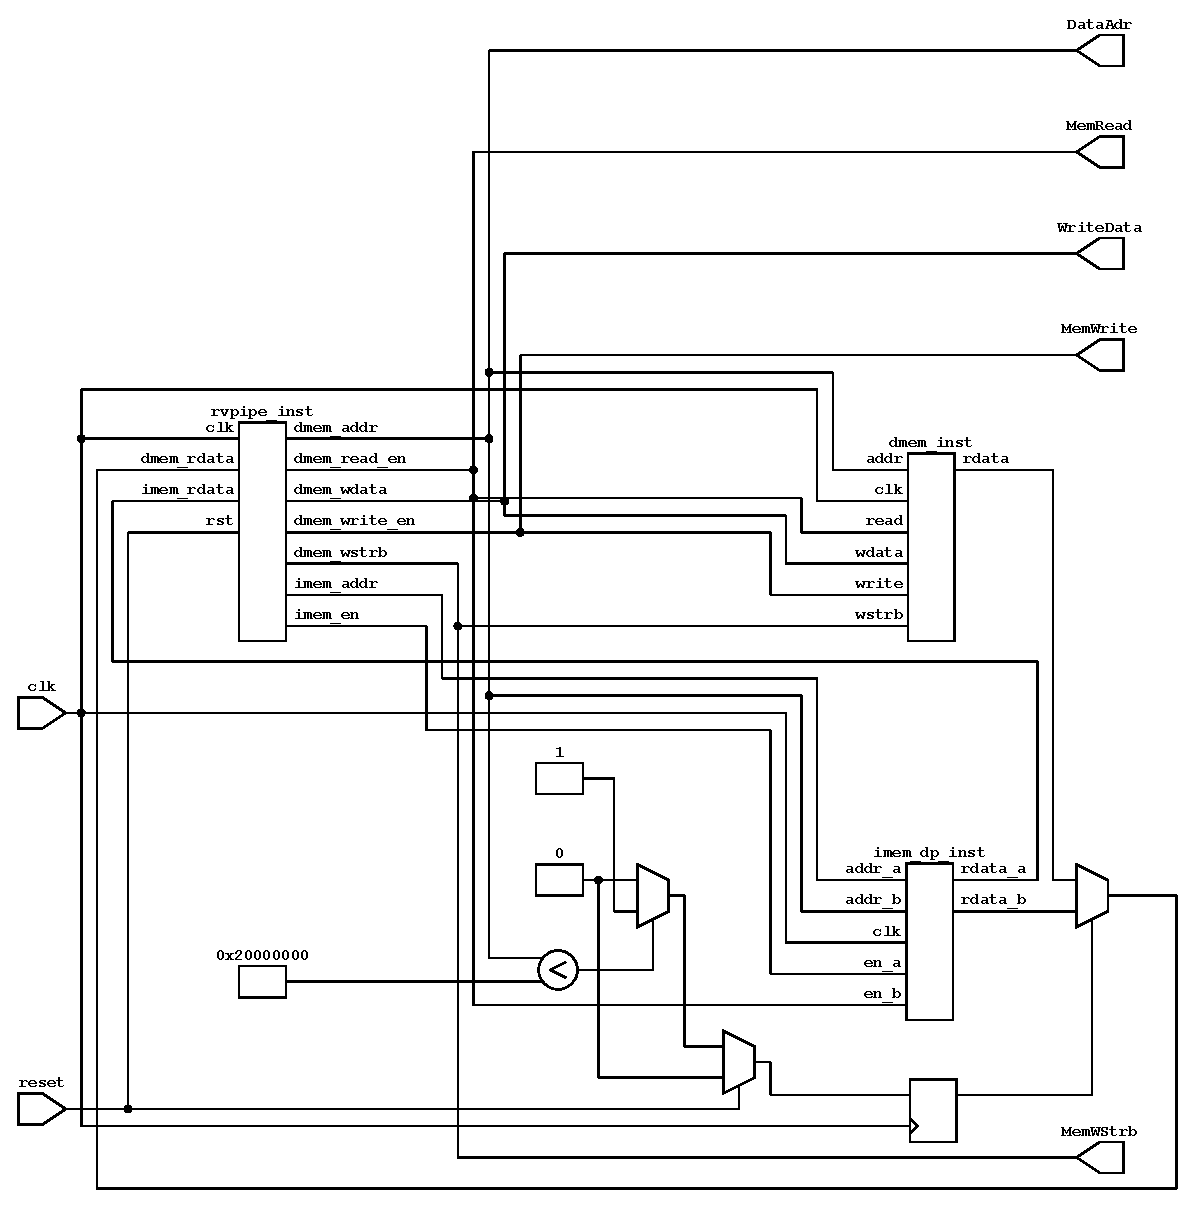
\includegraphics[width=0.62\linewidth]{uarch_system.pdf}
  \caption{System level (\texttt{top}). The synthesis top wires the pipelined
  core (\texttt{rvpipe\_inst}) to a dual-port instruction memory
  (\texttt{imem\_dp\_inst}) and a data memory (\texttt{dmem\_inst}); the dual-port
  IMEM also serves \texttt{.rodata} reads on port~B. Auto-generated with
  \texttt{netlistsvg}.}
  \label{fig:uarch-system}
\end{figure}

\begin{figure}[t]
  \centering
  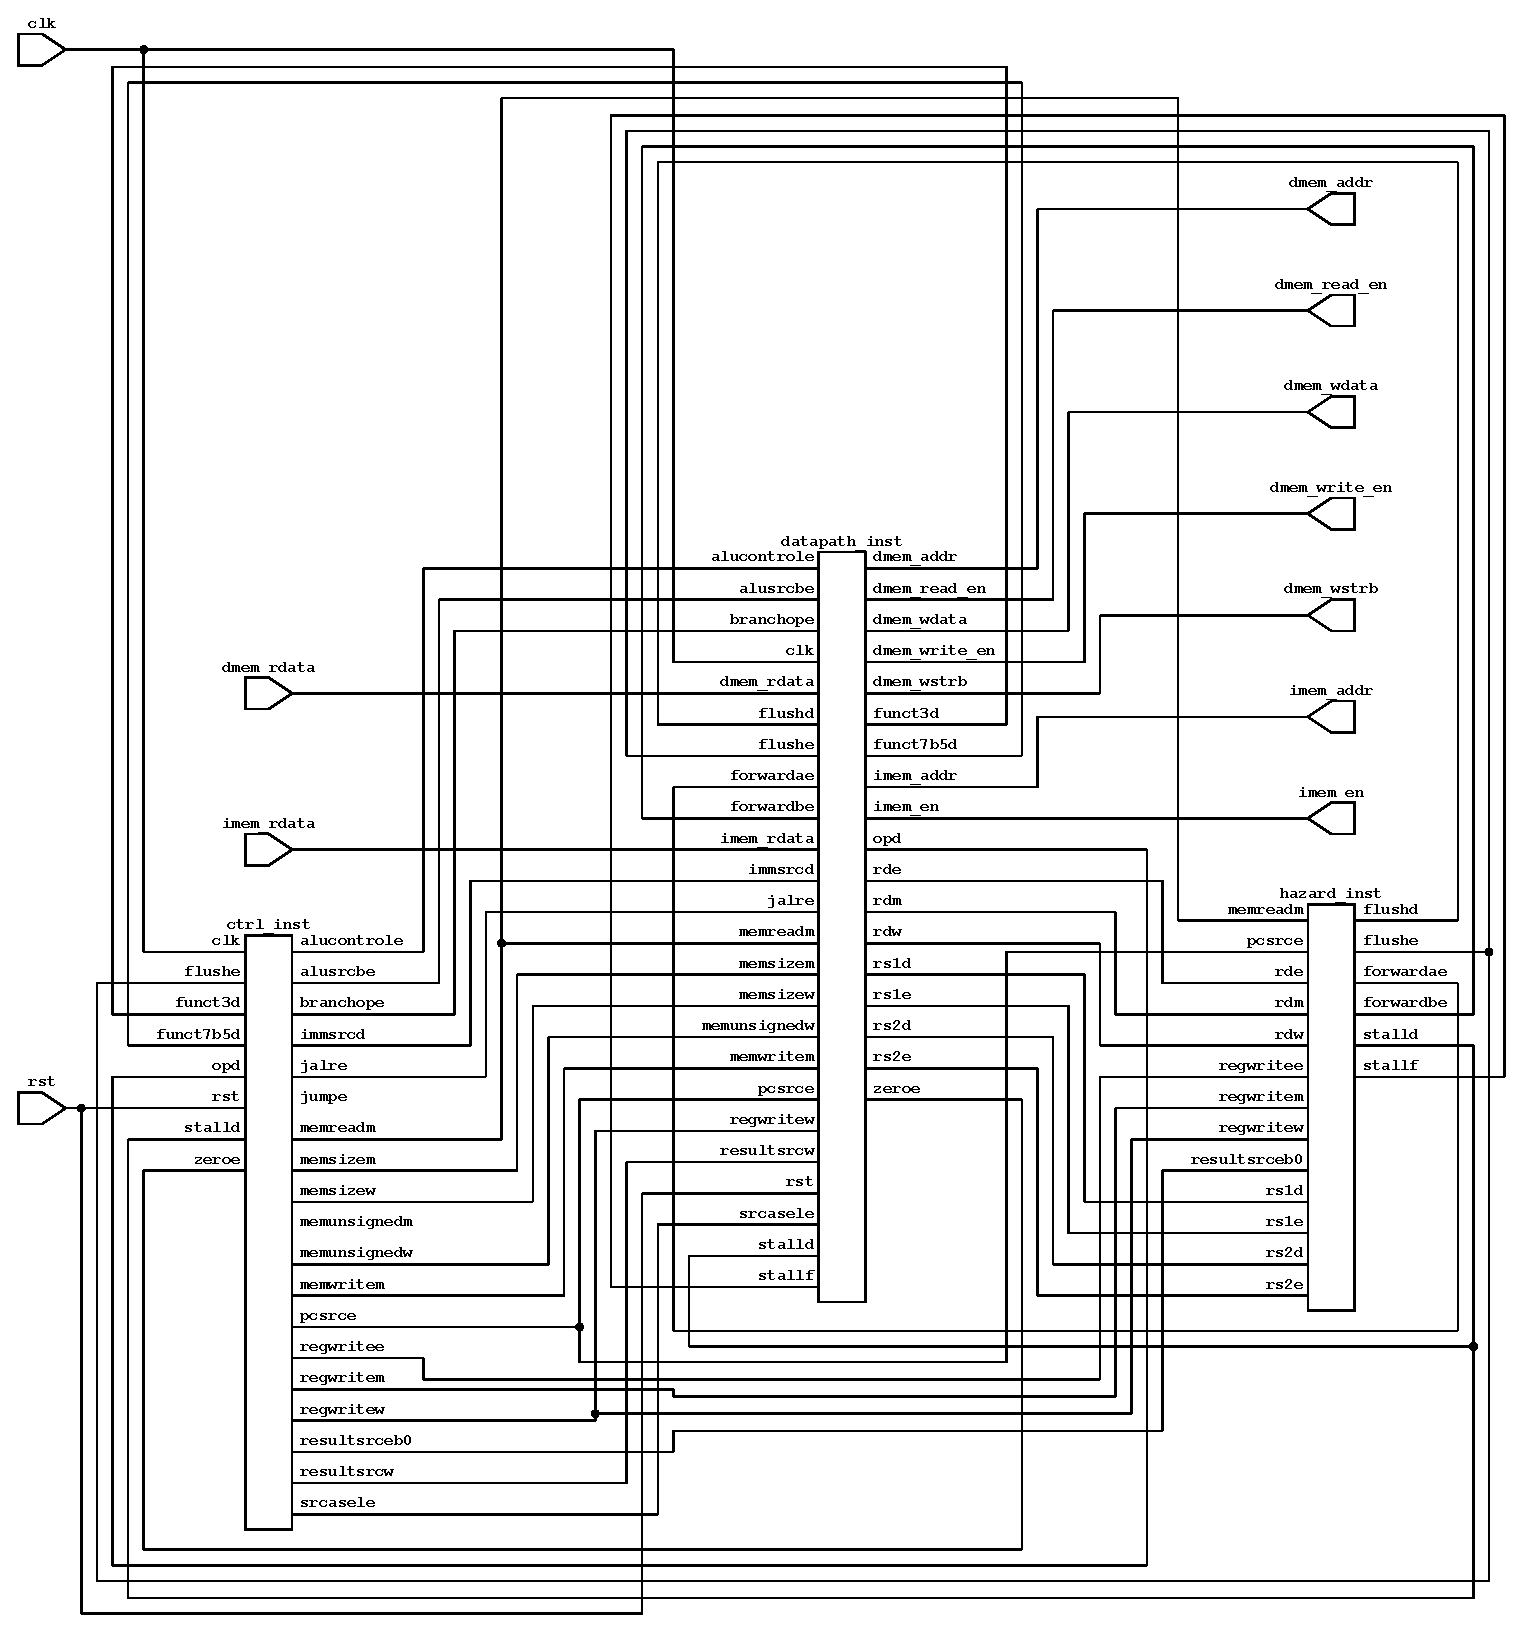
\includegraphics[width=\linewidth]{uarch_core.pdf}
  \caption{Core level (\texttt{riscvpipe}). The pipelined core binds the
  controller (\texttt{ctrl\_inst}), the structural datapath
  (\texttt{datapath\_inst}), and the hazard unit (\texttt{hazard\_inst}); the
  control and hazard nets between them are visible as the inter-block wiring.
  Auto-generated with \texttt{netlistsvg}.}
  \label{fig:uarch-core}
\end{figure}

\subsection{One detail that matters on FPGA: synchronous memories}
Instruction and data memories are written in a BRAM-friendly style with
synchronous reads. As a result, the registered memory outputs naturally align
with pipeline stage boundaries: the IMEM output provides \texttt{InstrD} and the
DMEM output provides \texttt{ReadDataW}. A small \texttt{flush\_d\_hold} mechanism
inserts a NOP after redirects to implement a textbook-style decode flush even
though BRAM outputs cannot be ``overwritten'' like a conventional F$\rightarrow$D
register.

\subsection{Stage-by-stage summary}
\begin{description}[leftmargin=*,labelwidth=2.2cm]
  \item[Fetch (F)] A \texttt{PCF} register feeds the instruction memory address.
  Next-PC selection chooses \texttt{PC+4} or an Execute-stage redirect
  (taken branch/jump or JALR).
  \item[Decode (D)] The controller decodes opcode/funct fields and the register
  file reads \texttt{rs1}/\texttt{rs2}. Immediate expansion produces
  \texttt{ImmExtD}. Decode-stage pipeline state supports stall/flush.
  \item[Execute (E)] The ALU runs with forwarded operands; a branch unit evaluates
  all RV32I branch types. Redirect decisions occur here and trigger flush of
  wrong-path work.
  \item[Memory (M)] The address and store data are registered; a memory access
  helper produces byte strobes and aligned store data for SB/SH/SW.
  \item[Writeback (W)] Load sign/zero extension is applied in W, the writeback mux
  selects ALU vs memory vs PC+4, and the register file writes on the rising edge
  with a small combinational bypass to resolve same-cycle W$\rightarrow$D read-after-write.
\end{description}

\begin{figure}[p]
  \centering
  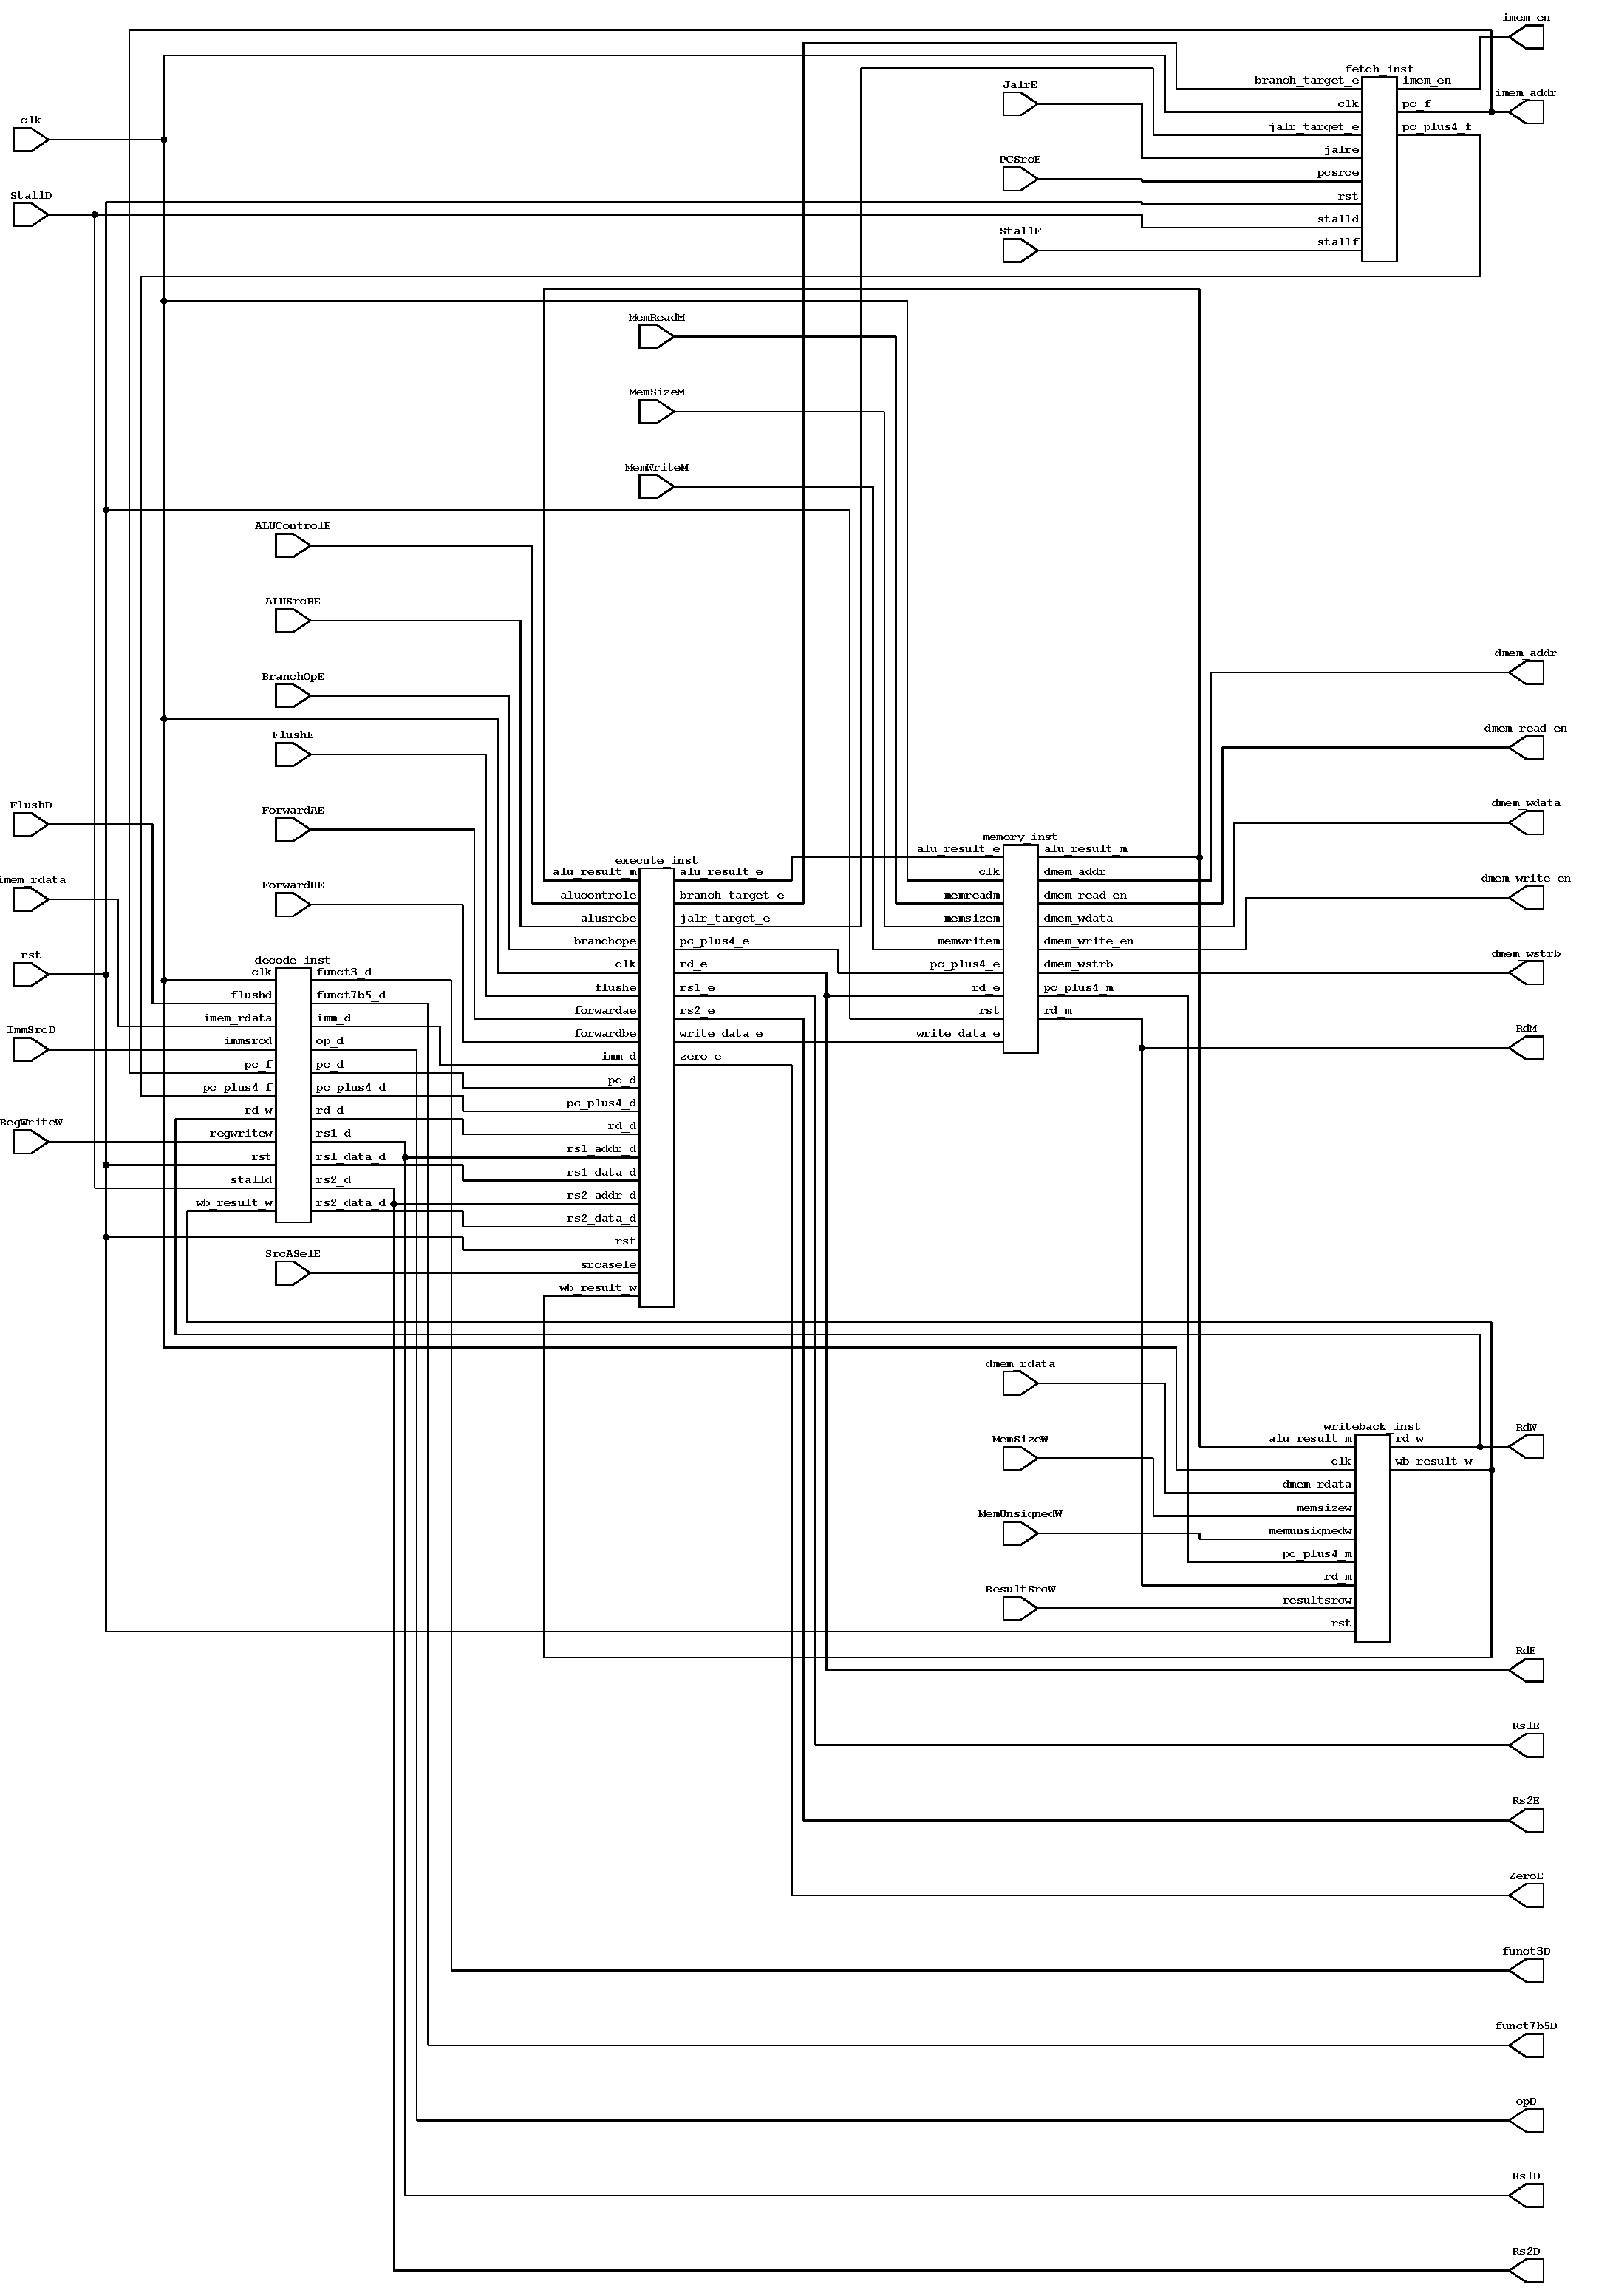
\includegraphics[width=\linewidth,height=0.88\textheight,keepaspectratio]{uarch_stages.pdf}
  \caption{Datapath stages (\texttt{datapath\_pipe}). The purely structural
  datapath instantiates the five per-stage wrappers (\texttt{fetch\_inst},
  \texttt{decode\_inst}, \texttt{execute\_inst}, \texttt{memory\_inst},
  \texttt{writeback\_inst}) and wires the inter-stage signals between them.
  Auto-generated with \texttt{netlistsvg}.}
  \label{fig:uarch-stages}
\end{figure}

\begin{figure}[p]
  \centering
  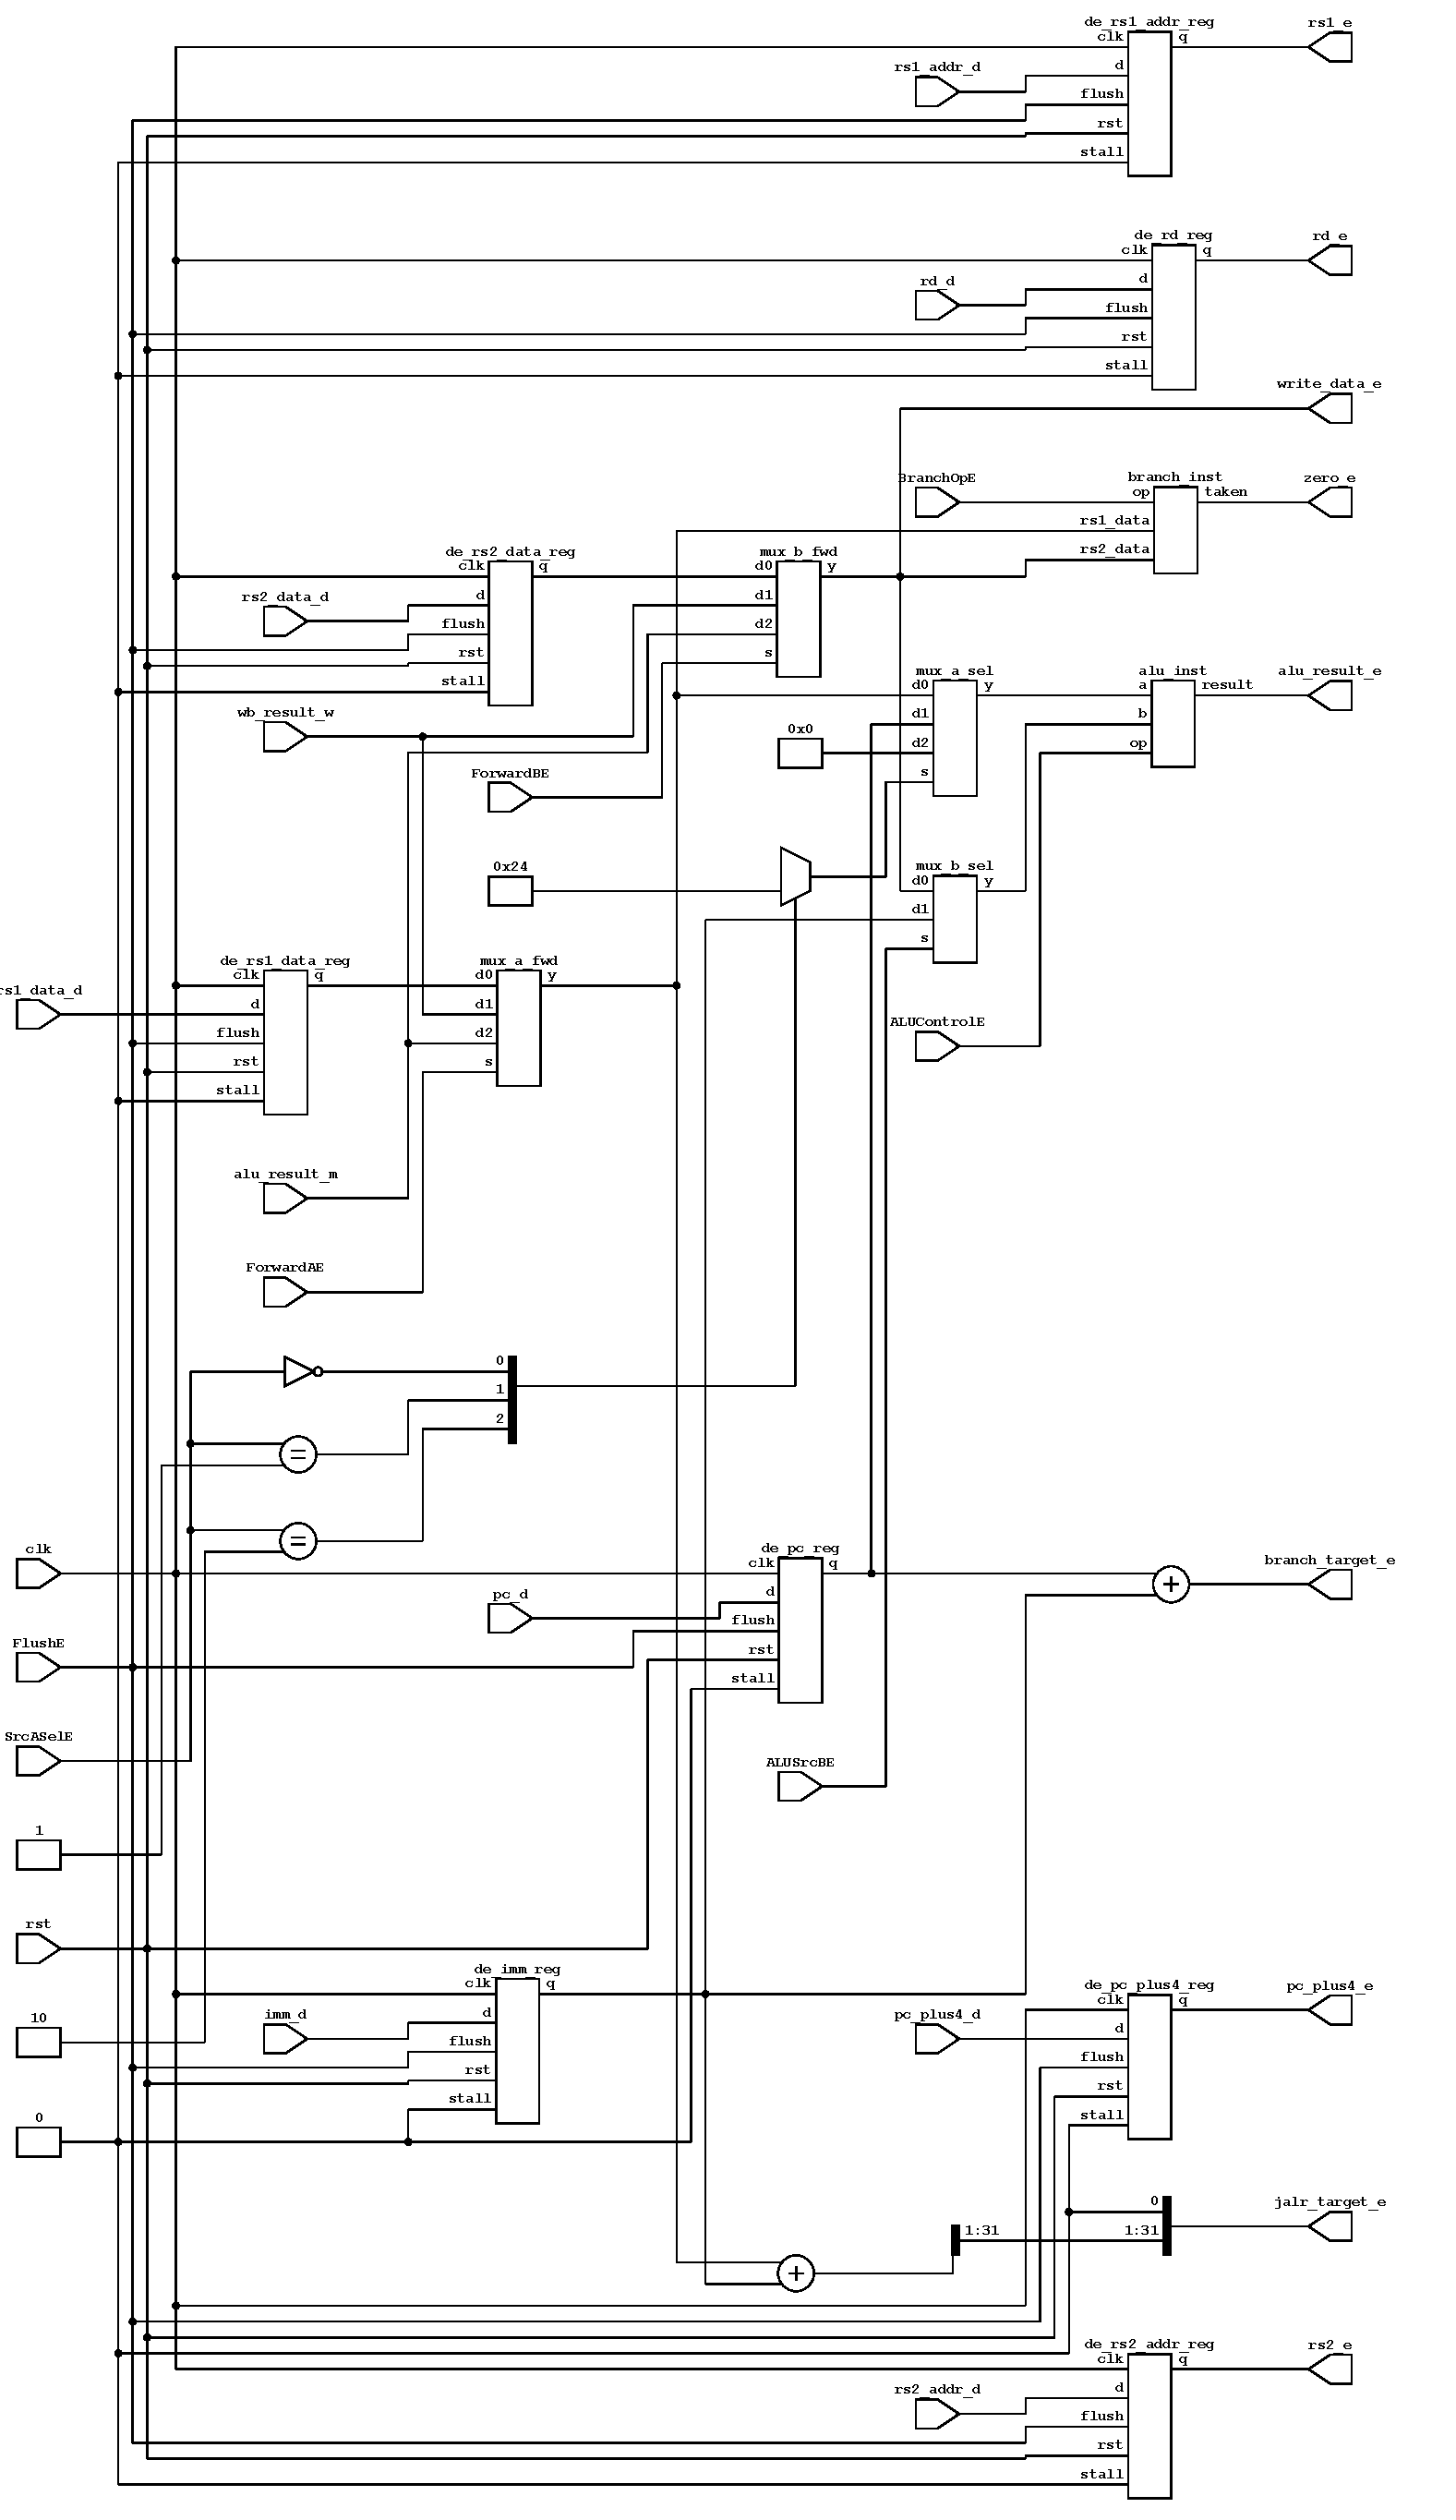
\includegraphics[width=\linewidth,height=0.88\textheight,keepaspectratio]{uarch_execute.pdf}
  \caption{Execute-stage internals (\texttt{execute\_stage}), showing the named
  functional units: the ALU (\texttt{alu\_inst}), the branch unit
  (\texttt{branch\_inst}), the forwarding and operand-select muxes
  (\texttt{mux\_a\_fwd}/\texttt{mux\_b\_fwd}, \texttt{mux\_a\_sel}/\texttt{mux\_b\_sel}),
  the D$\rightarrow$E pipeline registers (\texttt{de\_*\_reg}), and the
  branch-target adder. Auto-generated with \texttt{netlistsvg}.}
  \label{fig:uarch-execute}
\end{figure}

\paragraph{Per-instruction stage walkthrough}
The repository keeps a stage-by-stage walkthrough for each supported RV32I
instruction group in \texttt{docs/instruction\_control.md}. This PDF references
that Markdown source to avoid duplicating the same table-level material in two
places.

\subsection{Major RTL blocks (module map)}
At the core level, \texttt{riscvpipe} binds three blocks
(Figure~\ref{fig:uarch-core}): the controller, the structural datapath, and the
hazard unit.

The design is intentionally modular:
\begin{itemize}[leftmargin=*]
  \item \texttt{riscvpipe.vhd}: binds controller, datapath, and hazard unit into the pipelined core.
  \item \texttt{top.vhd}: wires the core to Harvard IMEM/DMEM models, including \texttt{.rodata} reads via dual-port IMEM. Exposes textbook observation ports (\texttt{DataAdr}, \texttt{WriteData}, \texttt{MemWrite}, \texttt{MemRead}, \texttt{MemWStrb}) so the VHDL testbench can monitor memory traffic directly.
  \item \texttt{fpga\_top.vhd}: thin Vivado synthesis wrapper around \texttt{top}. Exposes \texttt{clk}, \texttt{reset}, and a 1-bit \texttt{led} activity indicator (the MSB of a free-running blink counter XORed with an XOR reduction of every observation signal; the counter makes the LED blink while the clock runs, and the XOR fold prevents Vivado from eliminating the datapath as dead code). It also makes the core clock from the board clock with an MMCM (the FPGA's clock generator block; by default 80\,MHz on Basys3 and ZedBoard). The FPGA pad ring stays at 3 IOs; internal observation nets remain accessible via ILA with \texttt{MARK\_DEBUG}.
  \item \texttt{controller\_pipe.vhd}: decode in D; registers control into E/M/W.
  \item \texttt{datapath\_pipe.vhd}: \textbf{structural} top-level datapath that instantiates five per-stage wrapper entities and wires inter-stage signals (no inline processes or logic).
  \item \texttt{hazard\_unit.vhd}: forwarding, load-use stalls, and control-hazard flush.
  \item \texttt{imem\_dp.vhd}, \texttt{dmem.vhd}: synchronous-read memories coded to infer FPGA BRAM.
  \item \texttt{mem\_access\_unit.vhd}: SB/SH/SW byte strobes + store alignment.
  \item \texttt{load\_extend\_unit.vhd}: combinational load-data sign/zero extension applied in W.
\end{itemize}

\paragraph{Datapath stage hierarchy}
\texttt{datapath\_pipe.vhd} instantiates the following stage wrappers, each
containing named entity instances for pipeline registers (\texttt{pipe\_reg}),
muxes, and functional units.  This produces a navigable per-stage hierarchy in
Vivado's elaborated design view.
\begin{description}[leftmargin=*,labelwidth=3.2cm]
  \item[\texttt{fetch\_stage}] PC register (\texttt{pipe\_reg}), PC+4 adder, next-PC muxes, BRAM read-enable.
  \item[\texttt{decode\_stage}] F$\rightarrow$D pipeline registers, NOP insertion (\texttt{flush\_d\_hold}), \texttt{regfile}, \texttt{extend}.
  \item[\texttt{execute\_stage}] D$\rightarrow$E pipeline registers, forwarding \texttt{mux3} instances, ALU-B \texttt{mux2}, \texttt{alu}, \texttt{branch\_unit}, target computation.
  \item[\texttt{memory\_stage}] E$\rightarrow$M pipeline registers, \texttt{mem\_access\_unit}.
  \item[\texttt{writeback\_stage}] M$\rightarrow$W pipeline registers, \texttt{load\_extend\_unit}, WB result \texttt{mux3}.
\end{description}
A reusable \texttt{pipe\_reg} entity (generic \texttt{WIDTH}, ports for
\texttt{clk/rst/flush/stall/d/q}) implements all explicit pipeline registers.

\subsection{Hazard unit operation}
The hazard unit resolves the three hazard classes of a 5-stage pipeline. A
single elaboration-time generic, \texttt{FORWARDING\_ENABLE}, selects one of
two mutually exclusive bodies through an \texttt{if \ldots generate}. The
stall and flush \emph{outputs} (\texttt{StallF}, \texttt{StallD},
\texttt{FlushD}, \texttt{FlushE}) are produced by shared logic that is
identical in both modes; only the internal stall condition
(\texttt{stallD\_i}) and the forwarding muxes differ between them. The goal of
this subsection is to explain \emph{why each condition is required}, not merely
what it computes.

\subsubsection{Forwarding-enabled mode}
The operand-forwarding muxes choose, for the instruction in Execute, where each
ALU input comes from:

\begin{center}
\begin{tabular}{@{}llp{0.52\textwidth}@{}}
\toprule
Select & Source & Asserted when \\
\midrule
\texttt{"00"} & register file & no hazard, or source is \texttt{x0} (default) \\
\texttt{"10"} & \texttt{ALUResultM} & \texttt{RsxE=RdM} and \texttt{RegWriteM='1'} and \texttt{MemReadM='0'} and \texttt{RsxE/=x0} \\
\texttt{"01"} & \texttt{ResultW}    & \texttt{RsxE=RdW} and \texttt{RegWriteW='1'} and \texttt{RsxE/=x0} \\
\bottomrule
\end{tabular}
\end{center}

\begin{itemize}[leftmargin=*]
  \item \textbf{M before W priority.} When the same register is in flight in
  both M and W, the copy in M is the newer write and must win; the
  \texttt{if/elsif} order encodes this.
  \item \textbf{\texttt{MemReadM='0'} on the M path.} A load in M holds only the
  computed \emph{address} in \texttt{ALUResultM}, not its data; forwarding it
  would corrupt the operand. Loads are instead covered by the load-use stall,
  after which the value forwards safely from W. The W path needs no such guard,
  because W always carries the final committed value.
  \item \textbf{\texttt{RsxE/=x0}.} \texttt{x0} is hardwired to zero and is
  never a real dependency.
\end{itemize}

The remaining data hazard is the \emph{load-use} case: a load in E
(\texttt{ResultSrcEb0='1'}) produces its result only at the end of M, too late
to forward into the dependent instruction already in E. The unit stalls F and D
for one cycle and bubbles E; one cycle later the load is in W and forwards
normally:

\begin{lstlisting}[style=minrv]
stallD_i = ResultSrcEb0='1'
           and ( (Rs1D=RdE and Rs1D/=x0) or (Rs2D=RdE and Rs2D/=x0) )
\end{lstlisting}

\noindent The \texttt{/=x0} guards suppress a false stall when the consumer
reads \texttt{x0}.

\subsubsection{Stall-only mode}
For debugging and for demonstrating why forwarding matters, the unit can be
elaborated with \texttt{FORWARDING\_ENABLE=false}; the test scripts expose this.
The forwarding muxes are tied to \texttt{"00"} (the ALU always reads the
register file), so every RAW dependency must be resolved by stalling until the
producer writes back in W. \texttt{stallD\_i} becomes the OR of the load-use
term above and a generic RAW term:

\begin{lstlisting}[style=minrv]
rawStallD_b = (Rs1D=RdE or Rs2D=RdE) and RegWriteE='1' and RdE/=x0
           or (Rs1D=RdM or Rs2D=RdM) and RegWriteM='1' and RdM/=x0
           or (Rs1D=RdW or Rs2D=RdW) and RegWriteW='1' and RdW/=x0
\end{lstlisting}

\begin{itemize}[leftmargin=*]
  \item \textbf{\texttt{RegWrite*='1'}.} Stores and branches reuse the \texttt{Rd}
  bit-field for immediate bits, so a non-zero \texttt{Rd} does not imply a
  register write. Gating on the real control signal avoids stalling on
  non-existent dependencies.
  \item \textbf{\texttt{Rd*/=x0}.} A write to \texttt{x0} is discarded by the
  ISA, so an instruction whose destination is \texttt{x0} is not a producer.
\end{itemize}

\subsubsection{Shared stall and flush outputs}
\begin{lstlisting}[style=minrv]
StallF = stallD_i and not PCSrcE
StallD = stallD_i and not PCSrcE
FlushD = PCSrcE
FlushE = stallD_i or PCSrcE
\end{lstlisting}

\begin{itemize}[leftmargin=*]
  \item \texttt{StallF}/\texttt{StallD} freeze the PC and the F/D register so the
  dependent instruction stays in D until the hazard clears.
  \item \texttt{FlushD=PCSrcE} kills the speculatively fetched instruction in D
  when a branch or jump resolves taken in E.
  \item \texttt{FlushE} bubbles E for either reason: a data stall has frozen D
  (the instruction in E must not re-execute), or a taken branch must squash its
  wrong-path successor in E.
  \item \textbf{The \texttt{and not PCSrcE} guard.} When a taken branch coincides
  with a data stall the PC must still redirect. \texttt{StallF} is the only gate
  on the PC update -- there is no flush on the PC -- so the guard is
  \emph{required} on \texttt{StallF}; without it the PC freezes and the core
  re-fetches the wrong-path instruction indefinitely. On \texttt{StallD} the
  guard is \emph{redundant}: \texttt{FlushD=PCSrcE} already clears the F/D
  register, and \texttt{pipe\_reg} prioritises flush over stall
  (\texttt{rst/flush > stall > load}), so the register bubbles regardless of
  \texttt{StallD}; it is kept only for symmetry. In forwarding mode
  \texttt{stallD\_i} (a load in E) and \texttt{PCSrcE} (a taken branch/jump in E)
  are mutually exclusive, so the guard only ever fires in stall-only mode, where
  a \texttt{JAL}/\texttt{JALR} both writes \texttt{rd} and sets \texttt{PCSrcE}.
\end{itemize}
